% Created by tikzDevice version 0.12.6 on 2024-11-10 21:27:34
% !TEX encoding = UTF-8 Unicode
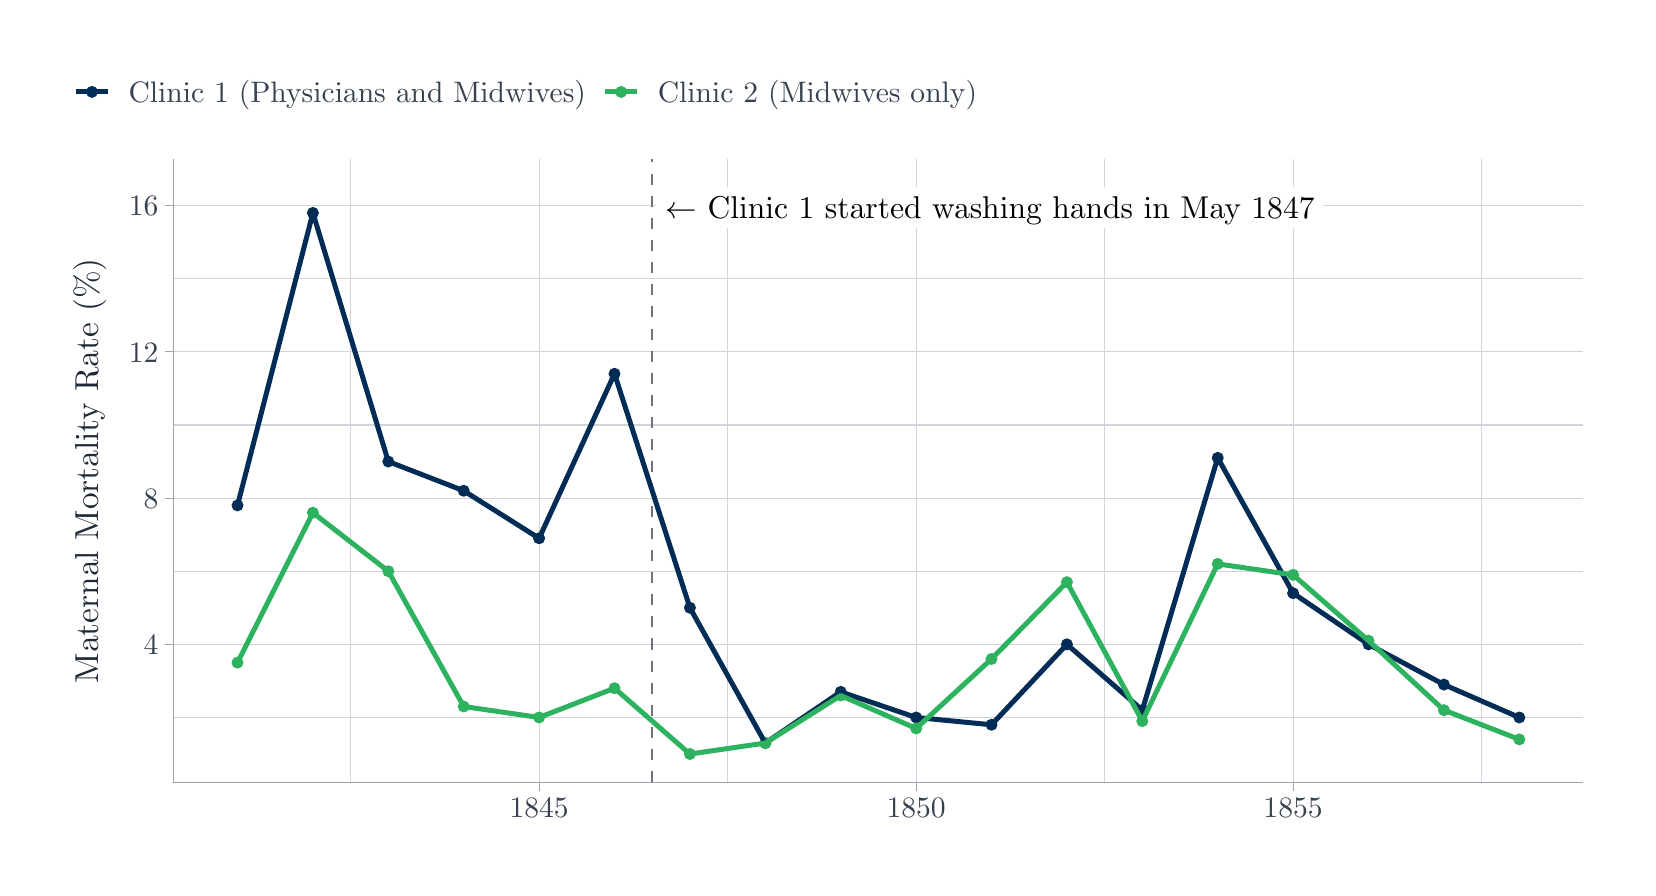
\begin{tikzpicture}[x=1pt,y=1pt]
\definecolor{fillColor}{RGB}{255,255,255}
\path[use as bounding box,fill=fillColor] (0,0) rectangle (578.16,303.53);
\begin{scope}
\path[clip] (  0.00,  0.00) rectangle (578.16,303.53);
\definecolor{drawColor}{RGB}{255,255,255}

\path[draw=drawColor,line width= 0.6pt,line join=round,line cap=round,fill=fillColor] (  0.00,  0.00) rectangle (578.16,303.53);
\end{scope}
\begin{scope}
\path[clip] ( 52.66, 30.82) rectangle (562.16,256.08);
\definecolor{drawColor}{RGB}{255,255,255}
\definecolor{fillColor}{RGB}{255,255,255}

\path[draw=drawColor,line width= 0.6pt,line join=round,line cap=round,fill=fillColor] ( 52.66, 30.82) rectangle (562.16,256.08);
\definecolor{drawColor}{RGB}{209,213,219}

\path[draw=drawColor,line width= 0.4pt,line join=round] ( 52.66, 54.27) --
	(562.16, 54.27);

\path[draw=drawColor,line width= 0.4pt,line join=round] ( 52.66,107.12) --
	(562.16,107.12);

\path[draw=drawColor,line width= 0.4pt,line join=round] ( 52.66,159.97) --
	(562.16,159.97);

\path[draw=drawColor,line width= 0.4pt,line join=round] ( 52.66,212.81) --
	(562.16,212.81);

\path[draw=drawColor,line width= 0.4pt,line join=round] (116.69, 30.82) --
	(116.69,256.08);

\path[draw=drawColor,line width= 0.4pt,line join=round] (252.92, 30.82) --
	(252.92,256.08);

\path[draw=drawColor,line width= 0.4pt,line join=round] (389.15, 30.82) --
	(389.15,256.08);

\path[draw=drawColor,line width= 0.4pt,line join=round] (525.38, 30.82) --
	(525.38,256.08);

\path[draw=drawColor,line width= 0.4pt,line join=round] ( 52.66, 80.70) --
	(562.16, 80.70);

\path[draw=drawColor,line width= 0.4pt,line join=round] ( 52.66,133.54) --
	(562.16,133.54);

\path[draw=drawColor,line width= 0.4pt,line join=round] ( 52.66,186.39) --
	(562.16,186.39);

\path[draw=drawColor,line width= 0.4pt,line join=round] ( 52.66,239.24) --
	(562.16,239.24);

\path[draw=drawColor,line width= 0.4pt,line join=round] (184.81, 30.82) --
	(184.81,256.08);

\path[draw=drawColor,line width= 0.4pt,line join=round] (321.04, 30.82) --
	(321.04,256.08);

\path[draw=drawColor,line width= 0.4pt,line join=round] (457.26, 30.82) --
	(457.26,256.08);
\definecolor{drawColor}{RGB}{113,113,122}

\path[draw=drawColor,line width= 0.6pt,dash pattern=on 4pt off 4pt ,line join=round] (225.68, 30.82) -- (225.68,256.08);

\path[fill=fillColor] (229.09,231.15) --
	(465.92,231.15) --
	(465.84,231.15) --
	(466.17,231.16) --
	(466.50,231.23) --
	(466.81,231.35) --
	(467.09,231.51) --
	(467.35,231.72) --
	(467.57,231.97) --
	(467.75,232.25) --
	(467.88,232.55) --
	(467.95,232.88) --
	(467.98,233.21) --
	(467.98,233.21) --
	(467.98,243.78) --
	(467.98,243.78) --
	(467.95,244.11) --
	(467.88,244.44) --
	(467.75,244.74) --
	(467.57,245.02) --
	(467.35,245.27) --
	(467.09,245.48) --
	(466.81,245.64) --
	(466.50,245.76) --
	(466.17,245.83) --
	(465.92,245.84) --
	(229.09,245.84) --
	(229.34,245.83) --
	(229.01,245.84) --
	(228.68,245.80) --
	(228.36,245.71) --
	(228.07,245.57) --
	(227.79,245.38) --
	(227.55,245.15) --
	(227.36,244.88) --
	(227.20,244.59) --
	(227.10,244.28) --
	(227.04,243.95) --
	(227.04,243.78) --
	(227.04,233.21) --
	(227.04,233.37) --
	(227.04,233.04) --
	(227.10,232.71) --
	(227.20,232.40) --
	(227.36,232.11) --
	(227.55,231.84) --
	(227.79,231.61) --
	(228.07,231.42) --
	(228.36,231.28) --
	(228.68,231.19) --
	(229.01,231.15) --
	cycle;
\end{scope}
\begin{scope}
\path[clip] ( 52.66, 30.82) rectangle (562.16,256.08);
\definecolor{drawColor}{RGB}{0,0,0}

\node[text=drawColor,anchor=base west,inner sep=0pt, outer sep=0pt, scale=  1.14] at (230.46,234.58) {$\leftarrow$ Clinic 1 started washing hands in May 1847};
\end{scope}
\begin{scope}
\path[clip] ( 52.66, 30.82) rectangle (562.16,256.08);
\definecolor{drawColor}{RGB}{0,44,85}
\definecolor{fillColor}{RGB}{0,44,85}

\path[draw=drawColor,line width= 0.4pt,line join=round,line cap=round,fill=fillColor] ( 75.82,130.90) circle (  1.96);

\path[draw=drawColor,line width= 0.4pt,line join=round,line cap=round,fill=fillColor] (103.07,236.59) circle (  1.96);

\path[draw=drawColor,line width= 0.4pt,line join=round,line cap=round,fill=fillColor] (130.32,146.75) circle (  1.96);

\path[draw=drawColor,line width= 0.4pt,line join=round,line cap=round,fill=fillColor] (157.56,136.19) circle (  1.96);

\path[draw=drawColor,line width= 0.4pt,line join=round,line cap=round,fill=fillColor] (184.81,119.01) circle (  1.96);

\path[draw=drawColor,line width= 0.4pt,line join=round,line cap=round,fill=fillColor] (212.05,178.46) circle (  1.96);

\path[draw=drawColor,line width= 0.4pt,line join=round,line cap=round,fill=fillColor] (239.30, 93.91) circle (  1.96);

\path[draw=drawColor,line width= 0.4pt,line join=round,line cap=round,fill=fillColor] (266.54, 45.03) circle (  1.96);

\path[draw=drawColor,line width= 0.4pt,line join=round,line cap=round,fill=fillColor] (293.79, 63.52) circle (  1.96);

\path[draw=drawColor,line width= 0.4pt,line join=round,line cap=round,fill=fillColor] (321.04, 54.27) circle (  1.96);

\path[draw=drawColor,line width= 0.4pt,line join=round,line cap=round,fill=fillColor] (348.28, 51.63) circle (  1.96);

\path[draw=drawColor,line width= 0.4pt,line join=round,line cap=round,fill=fillColor] (375.53, 80.70) circle (  1.96);

\path[draw=drawColor,line width= 0.4pt,line join=round,line cap=round,fill=fillColor] (402.77, 56.92) circle (  1.96);

\path[draw=drawColor,line width= 0.4pt,line join=round,line cap=round,fill=fillColor] (430.02,148.08) circle (  1.96);

\path[draw=drawColor,line width= 0.4pt,line join=round,line cap=round,fill=fillColor] (457.26, 99.19) circle (  1.96);

\path[draw=drawColor,line width= 0.4pt,line join=round,line cap=round,fill=fillColor] (484.51, 80.70) circle (  1.96);

\path[draw=drawColor,line width= 0.4pt,line join=round,line cap=round,fill=fillColor] (511.76, 66.16) circle (  1.96);

\path[draw=drawColor,line width= 0.4pt,line join=round,line cap=round,fill=fillColor] (539.00, 54.27) circle (  1.96);
\definecolor{drawColor}{RGB}{45,178,95}
\definecolor{fillColor}{RGB}{45,178,95}

\path[draw=drawColor,line width= 0.4pt,line join=round,line cap=round,fill=fillColor] ( 75.82, 74.09) circle (  1.96);

\path[draw=drawColor,line width= 0.4pt,line join=round,line cap=round,fill=fillColor] (103.07,128.26) circle (  1.96);

\path[draw=drawColor,line width= 0.4pt,line join=round,line cap=round,fill=fillColor] (130.32,107.12) circle (  1.96);

\path[draw=drawColor,line width= 0.4pt,line join=round,line cap=round,fill=fillColor] (157.56, 58.24) circle (  1.96);

\path[draw=drawColor,line width= 0.4pt,line join=round,line cap=round,fill=fillColor] (184.81, 54.27) circle (  1.96);

\path[draw=drawColor,line width= 0.4pt,line join=round,line cap=round,fill=fillColor] (212.05, 64.84) circle (  1.96);

\path[draw=drawColor,line width= 0.4pt,line join=round,line cap=round,fill=fillColor] (239.30, 41.06) circle (  1.96);

\path[draw=drawColor,line width= 0.4pt,line join=round,line cap=round,fill=fillColor] (266.54, 45.03) circle (  1.96);

\path[draw=drawColor,line width= 0.4pt,line join=round,line cap=round,fill=fillColor] (293.79, 62.20) circle (  1.96);

\path[draw=drawColor,line width= 0.4pt,line join=round,line cap=round,fill=fillColor] (321.04, 50.31) circle (  1.96);

\path[draw=drawColor,line width= 0.4pt,line join=round,line cap=round,fill=fillColor] (348.28, 75.41) circle (  1.96);

\path[draw=drawColor,line width= 0.4pt,line join=round,line cap=round,fill=fillColor] (375.53,103.16) circle (  1.96);

\path[draw=drawColor,line width= 0.4pt,line join=round,line cap=round,fill=fillColor] (402.77, 52.95) circle (  1.96);

\path[draw=drawColor,line width= 0.4pt,line join=round,line cap=round,fill=fillColor] (430.02,109.76) circle (  1.96);

\path[draw=drawColor,line width= 0.4pt,line join=round,line cap=round,fill=fillColor] (457.26,105.80) circle (  1.96);

\path[draw=drawColor,line width= 0.4pt,line join=round,line cap=round,fill=fillColor] (484.51, 82.02) circle (  1.96);

\path[draw=drawColor,line width= 0.4pt,line join=round,line cap=round,fill=fillColor] (511.76, 56.92) circle (  1.96);

\path[draw=drawColor,line width= 0.4pt,line join=round,line cap=round,fill=fillColor] (539.00, 46.35) circle (  1.96);
\definecolor{drawColor}{RGB}{0,44,85}

\path[draw=drawColor,line width= 1.8pt,line join=round] ( 75.82,130.90) --
	(103.07,236.59) --
	(130.32,146.75) --
	(157.56,136.19) --
	(184.81,119.01) --
	(212.05,178.46) --
	(239.30, 93.91) --
	(266.54, 45.03) --
	(293.79, 63.52) --
	(321.04, 54.27) --
	(348.28, 51.63) --
	(375.53, 80.70) --
	(402.77, 56.92) --
	(430.02,148.08) --
	(457.26, 99.19) --
	(484.51, 80.70) --
	(511.76, 66.16) --
	(539.00, 54.27);
\definecolor{drawColor}{RGB}{45,178,95}

\path[draw=drawColor,line width= 1.8pt,line join=round] ( 75.82, 74.09) --
	(103.07,128.26) --
	(130.32,107.12) --
	(157.56, 58.24) --
	(184.81, 54.27) --
	(212.05, 64.84) --
	(239.30, 41.06) --
	(266.54, 45.03) --
	(293.79, 62.20) --
	(321.04, 50.31) --
	(348.28, 75.41) --
	(375.53,103.16) --
	(402.77, 52.95) --
	(430.02,109.76) --
	(457.26,105.80) --
	(484.51, 82.02) --
	(511.76, 56.92) --
	(539.00, 46.35);
\end{scope}
\begin{scope}
\path[clip] (  0.00,  0.00) rectangle (578.16,303.53);
\definecolor{drawColor}{RGB}{156,163,175}

\path[draw=drawColor,line width= 0.3pt,line join=round] ( 52.66, 30.82) --
	( 52.66,256.08);
\end{scope}
\begin{scope}
\path[clip] (  0.00,  0.00) rectangle (578.16,303.53);
\definecolor{drawColor}{RGB}{55,65,81}

\node[text=drawColor,anchor=base east,inner sep=0pt, outer sep=0pt, scale=  1.07] at ( 47.26, 77.02) {4};

\node[text=drawColor,anchor=base east,inner sep=0pt, outer sep=0pt, scale=  1.07] at ( 47.26,129.87) {8};

\node[text=drawColor,anchor=base east,inner sep=0pt, outer sep=0pt, scale=  1.07] at ( 47.26,182.71) {12};

\node[text=drawColor,anchor=base east,inner sep=0pt, outer sep=0pt, scale=  1.07] at ( 47.26,235.56) {16};
\end{scope}
\begin{scope}
\path[clip] (  0.00,  0.00) rectangle (578.16,303.53);
\definecolor{drawColor}{RGB}{156,163,175}

\path[draw=drawColor,line width= 0.3pt,line join=round] ( 49.66, 80.70) --
	( 52.66, 80.70);

\path[draw=drawColor,line width= 0.3pt,line join=round] ( 49.66,133.54) --
	( 52.66,133.54);

\path[draw=drawColor,line width= 0.3pt,line join=round] ( 49.66,186.39) --
	( 52.66,186.39);

\path[draw=drawColor,line width= 0.3pt,line join=round] ( 49.66,239.24) --
	( 52.66,239.24);
\end{scope}
\begin{scope}
\path[clip] (  0.00,  0.00) rectangle (578.16,303.53);
\definecolor{drawColor}{RGB}{156,163,175}

\path[draw=drawColor,line width= 0.3pt,line join=round] ( 52.66, 30.82) --
	(562.16, 30.82);
\end{scope}
\begin{scope}
\path[clip] (  0.00,  0.00) rectangle (578.16,303.53);
\definecolor{drawColor}{RGB}{156,163,175}

\path[draw=drawColor,line width= 0.3pt,line join=round] (184.81, 27.82) --
	(184.81, 30.82);

\path[draw=drawColor,line width= 0.3pt,line join=round] (321.04, 27.82) --
	(321.04, 30.82);

\path[draw=drawColor,line width= 0.3pt,line join=round] (457.26, 27.82) --
	(457.26, 30.82);
\end{scope}
\begin{scope}
\path[clip] (  0.00,  0.00) rectangle (578.16,303.53);
\definecolor{drawColor}{RGB}{55,65,81}

\node[text=drawColor,anchor=base,inner sep=0pt, outer sep=0pt, scale=  1.07] at (184.81, 18.07) {1845};

\node[text=drawColor,anchor=base,inner sep=0pt, outer sep=0pt, scale=  1.07] at (321.04, 18.07) {1850};

\node[text=drawColor,anchor=base,inner sep=0pt, outer sep=0pt, scale=  1.07] at (457.26, 18.07) {1855};
\end{scope}
\begin{scope}
\path[clip] (  0.00,  0.00) rectangle (578.16,303.53);
\definecolor{drawColor}{RGB}{31,41,55}

\node[text=drawColor,rotate= 90.00,anchor=base,inner sep=0pt, outer sep=0pt, scale=  1.20] at ( 25.43,143.45) {Maternal Mortality Rate (\%)};
\end{scope}
\begin{scope}
\path[clip] (  0.00,  0.00) rectangle (578.16,303.53);
\definecolor{drawColor}{RGB}{255,255,255}
\definecolor{fillColor}{RGB}{255,255,255}

\path[draw=drawColor,line width= 0.6pt,line join=round,line cap=round,fill=fillColor] ( 16.00,268.08) rectangle (342.72,287.53);
\end{scope}
\begin{scope}
\path[clip] (  0.00,  0.00) rectangle (578.16,303.53);
\definecolor{drawColor}{RGB}{255,255,255}
\definecolor{fillColor}{RGB}{255,255,255}

\path[draw=drawColor,line width= 0.6pt,line join=round,line cap=round,fill=fillColor] ( 16.00,273.08) rectangle ( 30.45,287.53);
\end{scope}
\begin{scope}
\path[clip] (  0.00,  0.00) rectangle (578.16,303.53);
\definecolor{drawColor}{RGB}{0,44,85}
\definecolor{fillColor}{RGB}{0,44,85}

\path[draw=drawColor,line width= 0.4pt,line join=round,line cap=round,fill=fillColor] ( 23.23,280.31) circle (  1.96);
\end{scope}
\begin{scope}
\path[clip] (  0.00,  0.00) rectangle (578.16,303.53);
\definecolor{drawColor}{RGB}{0,44,85}

\path[draw=drawColor,line width= 1.8pt,line join=round] ( 17.45,280.31) -- ( 29.01,280.31);
\end{scope}
\begin{scope}
\path[clip] (  0.00,  0.00) rectangle (578.16,303.53);
\definecolor{drawColor}{RGB}{255,255,255}
\definecolor{fillColor}{RGB}{255,255,255}

\path[draw=drawColor,line width= 0.6pt,line join=round,line cap=round,fill=fillColor] (207.24,273.08) rectangle (221.69,287.53);
\end{scope}
\begin{scope}
\path[clip] (  0.00,  0.00) rectangle (578.16,303.53);
\definecolor{drawColor}{RGB}{45,178,95}
\definecolor{fillColor}{RGB}{45,178,95}

\path[draw=drawColor,line width= 0.4pt,line join=round,line cap=round,fill=fillColor] (214.46,280.31) circle (  1.96);
\end{scope}
\begin{scope}
\path[clip] (  0.00,  0.00) rectangle (578.16,303.53);
\definecolor{drawColor}{RGB}{45,178,95}

\path[draw=drawColor,line width= 1.8pt,line join=round] (208.68,280.31) -- (220.24,280.31);
\end{scope}
\begin{scope}
\path[clip] (  0.00,  0.00) rectangle (578.16,303.53);
\definecolor{drawColor}{RGB}{55,65,81}

\node[text=drawColor,anchor=base west,inner sep=0pt, outer sep=0pt, scale=  1.07] at ( 36.45,276.63) {Clinic 1 (Physicians and Midwives)};
\end{scope}
\begin{scope}
\path[clip] (  0.00,  0.00) rectangle (578.16,303.53);
\definecolor{drawColor}{RGB}{55,65,81}

\node[text=drawColor,anchor=base west,inner sep=0pt, outer sep=0pt, scale=  1.07] at (227.69,276.63) {Clinic 2 (Midwives only)};
\end{scope}
\end{tikzpicture}
